\documentclass[12pt]{extarticle}
\usepackage{tempora}
\usepackage[T1, T2A]{fontenc}
\usepackage[utf8]{inputenc}
\usepackage[english, ukrainian]{babel}
\usepackage{geometry}
\usepackage{graphicx}
\usepackage{multirow}
\usepackage{multicol}
\usepackage{float}
\graphicspath{{/home/artem/Pictures}}
\geometry
{
    a4paper,
    left=30mm,
    top=15mm,
    right=20mm,
    bottom=15mm,
}

\begin{document}
\begin{titlepage}
    \begin{center}
        \textbf{\normalsize{\MakeUppercase{
            Міністерство Освіти і науки України
            Національний університет "Львівська політехніка"
        }}}

        \begin{flushright}
        \textbf{ІКНІ}\\
        Кафедра \textbf{ПЗ}
        \end{flushright}
        \vspace{15mm}

        \includegraphics[width=0.4\textwidth]{lpnu_logo.png}

        \vspace*{\fill}

        \textbf{\normalsize{\MakeUppercase{Звіт}}}
            
        До лабораторної роботи №5

        \textbf{на тему:} “Опрацювання рядка символів з використанням ланцюжкових
        команд мікропроцесорів х86. Робота з файлами”

        \textbf{з дисципліни:} “Архітектура комп’ютера”
            
        \vspace*{\fill}

        \begin{flushright}

            \textbf{Лектор:}\\
            доцент кафедри ПЗ\\
            Крук О.Г.\\
            \vspace{12pt}

            \textbf{Виконав:}\\
            студент групи ПЗ-24\\
            Губик А. С.\\
            \vspace{12pt}

            \textbf{Прийняв:}\\
            доцент кафедри ПЗ\\
            Задорожний І. М.\\
        \vspace{12pt}
        \end{flushright}

        Львів -- 2023
            
            
    \end{center}
\end{titlepage}

\textbf{Тема роботи:} Опрацювання рядка символів з використанням ланцюжкових
команд мікропроцесорів х86. Робота з файлами

\vspace{12pt}

\textbf{Мета роботи:} освоїти команди асемблера для роботи з рядками
символів; опанувати функції Win32 для роботи з файлами; розвинути навики
складання програми для опрацювання рядка символів та програми для
створення, записування і читання текстового файла; відтранслювати і виконати
в режимі відлагодження програми, складені відповідно до свого індивідуального
завдання.

\subsection*{Індивідуальне завдання}
\begin{center}
    \begin{tabular}{| c | c |}
        \hline
        Варіант & Послідовність\\
        \hline
           3  & П7, П4, П1, П2, П3, П6, П5\\
        \hline
   
    \end{tabular}
\end{center}

\subsection*{Теоретичні відомості}
І. Команди оброблення рядкових примітивів
В системі команд процесорів Intel передбачено п'ять груп команд для
оброблення масивів байтів, слів та подвійних слів. Незважаючи на те, що всі вони
називаються рядковими примітивами, область їх використання не обмежується
тільки масивами рядків. З огляду на це доцільніше використовувати їх іншу
назву – ланцюжкові команди.
Для адресації пам'яті в цих командах використовуються регістри ESI та
EDI. Особливість цих команд полягає в тому, що обидва операнди розташовані
в пам'яті. При обробленні рядкових примітивів ці команди можуть автоматично
повторюватися, що робить їх застосування особливо зручним для роботи з
довгими рядками та масивами.
При роботі програми в захищеному режимі адресація пам'яті в командах
оброблення рядкових примітивів може здійснюватися через регістри ESI або
EDI. При цьому зміщення, що міститься в регістрі ESI, відраховується відносно
сегмента, чий дескриптор вказаний в регістрі DS, а зміщення, вказане в регістрі
EDI, відраховується відносно сегмента, чий дескриптор вказаний в регістрі ES.
При використанні лінійної моделі пам'яті в сегментних регістрах DS та ES
міститься одне і те ж значення, яке в програмі неможна змінювати.
Використання префікса повторення. Самі по собі команди оброблення
рядкових примітивів виконують тільки одну операцію над байтом, словом або
подвійним словом пам'яті. Однак, якщо перед ними вказати префікс повторення,
виконання команди буде повторено стільки разів, скільки вказано в регістрі ЕСХ.
Тобто з допомогою префікса можна виконати оброблення цілого масиву за
допомогою всього однієї команди. Існує кілька типів префіксів повторення:
REP - Повторювати команду, поки ЕСХ> 0;
REPZ, REPE - Повторювати команду, поки ЕСХ > 0 і прапорець нуля
установлений (ZF = 1);
REPNZ, REPNE - Повторювати команду, поки ЕСХ > 0 і прапорець нуля
скинутий (ZF = 0).
Прапорець напрямку DF. Стан цього прапорця впливає на те, який
напрямок переміщення по рядку і як в процесі виконання команд оброблення
рядкових примітивів змінюються значення регістрів ESI та EDI. Якщо прапорець
DF скинутий (напрямок - прямий), вони збільшуються на розмір оброблюваного 
операнда (1, 2 або 4 байти), а якщо встановлений (напрямок - зворотний), то
відповідно зменшуються.
Значення прапорця напрямку DF можна явно задати за допомогою команд
CLD та STD:
CLD ; Скидає прапорець напрямку DF (напрямок – прямий)
STD ; Встановлює прапорець напрямку DF (напрямок - зворотний)
(register).
\subsection*{Хід роботи}
\paragraph{1.}Перша програма

\begin{verbatim}
    INCLUDE Irvine\Irvine32.inc

    .data
    
    zeroBytes byte 0dh, 0ah
    
    firstText	byte	"   Artem  Hubyk       Serhiiovych   \   
    15-02-2005    Kobylovoloky   Ternopilska        PZ-24     ", 00
    secondText	byte	123 DUP (?)
    thirdText	byte	93 DUP (?)
    
    firstLen	DD		96
    secondLen	DD		126
    thirdLen	DD		96
    
    
    lastName	byte	24 DUP (?)
    foreName	byte	24 DUP (?)
    paternal	byte	24 DUP (?)
    birth		byte	24 DUP (?)
    city		byte	24 DUP (?)
    oblast		byte	24 DUP (?)
    Class		byte	24 DUP (?)
    
    lastNameLen	DD 0
    foreNameLen	DD 0 
    paternalLen	DD 0
    birthLen	DD 0
    cityLen		DD 0
    oblastLen	DD 0
    classLen	DD 0
    
    begin		DD 0
    spacesNum	DD 0
    MNumber 	DD 0
    
    
    
    filename	BYTE "hubyk.txt", 00
    fileHandle	DD ?
    byteCount	DD ?
    
    toAppend	byte "OOP - 88, Physics - 69", 00
    toAppendLen	DD 23
    
    
    
    .code
    
    spaceLen proc start:dword 
        lea edi, firstText
        add edi, start			;
        mov esi, edi
        mov eax, ' '
        mov ecx, firstLen		;
        cld
        repe scasb				;
        dec edi					;
        sub edi, esi			;
        mov eax, edi			;
        add ebx, eax			;
        mov begin, ebx			;
        ret
    spaceLen endp
    
    
    fieldLen proc start:dword
        lea edi, firstText
        add edi, start			
        mov esi, edi
        mov eax, ' '
        mov ecx, firstLen		;
        repne scasb				
        dec edi					
        sub edi, esi			
        mov eax, edi			
        mov ebx, eax			;
        add ebx, start			;
        ret
    fieldLen endp
    
    
    main proc
    
    
    
    mov ebx, 0
     
    invoke spaceLen, ebx ; lastName
    add spacesNum, eax
    invoke fieldLen, ebx
    mov foreNameLen, eax
    
    mov ecx, foreNameLen
    lea esi, firstText
    add esi, begin				
    lea edi, foreName
    rep movsb					
    
    
    invoke spaceLen, ebx ; foreName
    add spacesNum, eax
    invoke fieldLen, ebx
    mov lastNameLen, eax
    
    mov ecx, lastNameLen
    lea esi, firstText
    add esi, begin
    lea edi, lastName
    rep movsb
    
    
    invoke spaceLen, ebx ; paternal
    add spacesNum, eax
    invoke fieldLen, ebx
    mov paternalLen, eax
    
    mov ecx, paternalLen
    lea esi, firstText
    add esi, begin
    lea edi, paternal
    rep movsb
    
    
    invoke spaceLen, ebx ; birth
    add spacesNum, eax
    invoke fieldLen, ebx
    mov birthLen, eax
    
    mov ecx, birthLen
    lea esi, firstText
    add esi, begin
    lea edi, birth
    rep movsb
    
    
    invoke spaceLen, ebx ; city
    add spacesNum, eax
    invoke fieldLen, ebx
    mov cityLen, eax
    
    mov ecx, cityLen
    lea esi, firstText
    add esi, begin
    lea edi, city
    rep movsb
    
    
    invoke spaceLen, ebx ; oblast
    add spacesNum, eax
    invoke fieldLen, ebx
    mov oblastLen, eax
    
    mov ecx, oblastLen
    lea esi, firstText
    add esi, begin
    lea edi, oblast
    rep movsb
    
    invoke spaceLen, ebx ; class
    add spacesNum, eax
    invoke fieldLen, ebx
    mov classLen, eax
    
    mov ecx, classLen
    lea esi, firstText
    add esi, begin
    lea edi, Class
    rep movsb
    
    invoke spaceLen, ebx				
    add spacesNum, eax
    

    


    
    lea edi, secondText
    mov eax, ' '
    
    mov ecx, 7 ; Class
    rep stosb
    lea esi, Class
    mov ecx, classLen
    rep movsb
    
    mov ecx, 4 ; birth
    rep stosb
    lea esi, birth
    mov ecx, birthLen
    rep movsb
    
    mov ecx, 1 ; lastName
    rep stosb
    lea esi, lastName
    mov ecx, lastNameLen
    rep movsb
    
    mov ecx, 2 ; foreName
    rep stosb
    lea esi, foreName
    mov ecx, foreNameLen
    rep movsb
    
    mov ecx, 3 ; paternal
    rep stosb
    lea esi, paternal
    mov ecx, paternalLen
    rep movsb
    
    mov ecx, 6 ; oblast
    rep stosb
    lea esi, oblast
    mov ecx, oblastLen
    rep movsb
    
    mov ecx, 5 ; city
    rep stosb
    lea esi, city
    mov ecx, cityLen
    rep movsb
    
    lea esi, zeroBytes 
    mov ecx, 2
    rep movsb
    
    
    lea edx, secondText
    
    
    call WriteString
    
    
    invoke	CreateFile, ADDR filename, GENERIC_WRITE, DO_NOT_SHARE, NULL, 
            CREATE_ALWAYS, FILE_ATTRIBUTE_NORMAL, 0 ;
    mov fileHandle, eax
    
    INVOKE WriteFile, fileHandle, ADDR secondText, secondLen, ADDR byteCount, 0 ;
    INVOKE WriteFile, fileHandle, ADDR firstText, firstLen, ADDR byteCount, 0
    INVOKE CloseHandle, fileHandle
    
    
    invoke	CreateFile, ADDR filename, GENERIC_READ or GENERIC_WRITE, DO_NOT_SHARE, NULL, 
            OPEN_EXISTING, FILE_ATTRIBUTE_NORMAL, 0 
    
    mov fileHandle, eax
    
    INVOKE SetFilePointer, fileHandle, secondLen, 0, FILE_BEGIN 
    INVOKE ReadFile, fileHandle, ADDR thirdText, firstLen, ADDR byteCount, 0
    
    lea esi, thirdText
    mov ecx, thirdLen
    
    count: 
        lodsb
        cmp eax, 'A'
        jnz pass_increment
        inc MNumber
        pass_increment:
        loop count
    
    INVOKE SetFilePointer, fileHandle, 0, 0, FILE_END
    INVOKE WriteFile, fileHandle, ADDR toAppend, toAppendLen, ADDR byteCount, 0 
    INVOKE CloseHandle, fileHandle
    
    
    Invoke ExitProcess, 0
    
    
    ret
    main ENDP
    end main

\end{verbatim}

\vspace{12pt}
\begin{figure}[H]
    \centering
    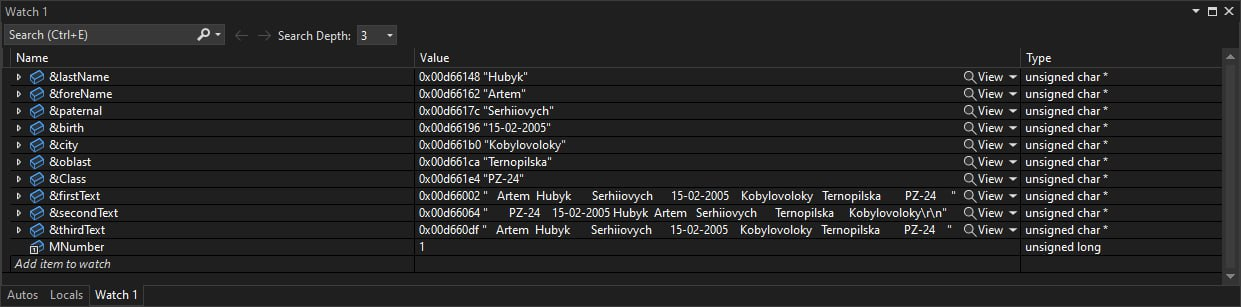
\includegraphics[width=0.90\textwidth]{var.jpg}
    \caption{Транспонування матриці}
\end{figure}
\begin{figure}[H]
    \centering
    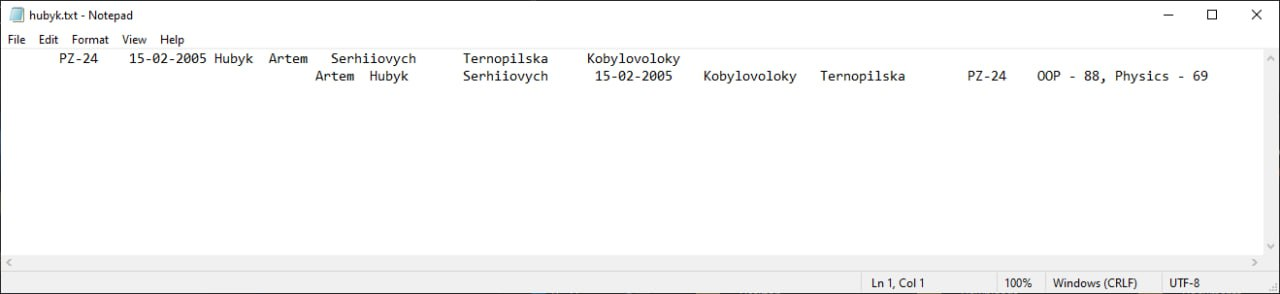
\includegraphics[width=0.90\textwidth]{file.jpg}
    \caption{Змінні}
\end{figure}

\begin{figure}[H]
    \centering
    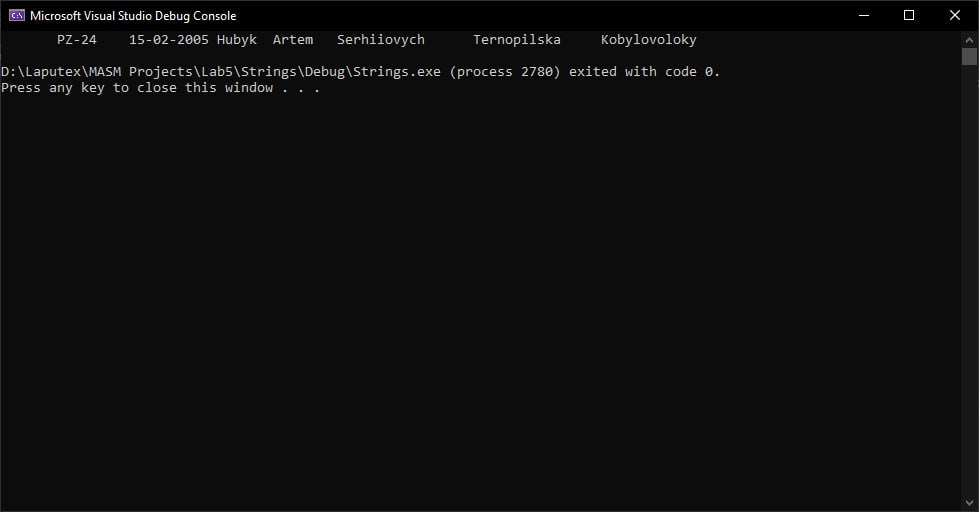
\includegraphics[width=0.90\textwidth]{console.jpg}
    \caption{Перша ітерація}
\end{figure}

\vspace{12pt}

\subsection*{Висновок} 
Я навчився працювати з файлами і вводом-виводом, а
бібліотека ірвін дає можливість полегшити цю роботу.


\end{document}